\section{Lightning Illumination Model}
\label{section:input_power}
%\subsection{Emission Spectrum}
A single lightning flash is a stochastic dielectric breakdown process. While a terrestrial lightning flash consists of several repeated strokes at varying incident angles, we adopt the simplified model used by \citealt{Lauben1998}, \citealt{Bortnik2005}, and subsequent workers.

The lightning flash is modeled as a single, vertical current pulse from a height $H_E$, with a time profile given by equation \ref{eqn:td_pulse}:
\begin{equation}
\label{eqn:td_pulse}
I(t)=I_0(e^{-a t} - e^{-b t})
\end{equation}

We relate the time-domain current profile to radiated power using the far-field approximation for an arbitrary source, given by \cite{Griffiths1999}, page 457:
\begin{equation}
\label{eqn:griffiths_power}
S(t) \approx \frac{1}{\mu_0}(\mathbf{E} \times \mathbf{B}) = \frac{\mu_0}{16\pi^2c}\left[\ddot{p}(t)\right]^2 \left(\frac{\sin^2\theta}{r^2}\right)\mathbf{\hat{r}}
\end{equation}

where $p(t)$ is the dipole moment given by $p=2 H_E \int_0^t{I(t)}dt$, r is the distance from the flash in meters, and $\theta$ is the angle to the flash. Taking the second derivative of the dipole moment (the first derivative of the current profile) gives us the far-field time-domain power equation:

\begin{equation}
\label{eqn:farfield_power_td}
S(t) = \frac{1}{Z_0}\left(\frac{\mu_0 H_E I_0}{2 \pi}\right)^2\left(\frac{\sin^2\theta}{r^2}\right) \left(a e^{-a t} - b e^{-b t}\right)^2  \mathbf{\hat{r}}
\end{equation}

where we have used the relation $Z_0 = \mu_0 c$. Equation \ref{eqn:farfield_power_td} has units of energy flux density, Watts per square meter ($J/m^2/$sec).

To determine the frequency spectrum of the radiated power, we take the Fourier transform of equation \ref{eqn:farfield_power_td}:

\begin{equation}
\label{eqn:farfield_power_fd}
S(\omega) = \frac{1}{Z_0}\left(\frac{\mu_0 H_E I_0}{2 \pi}\right)^2\left(\frac{\sin^2\theta}{r^2}\right) \frac{\omega^2(a-b)^2}{(\omega^2 + a^2)(\omega^2 + b^2)}  \mathbf{\hat{r}}
\end{equation}

which has units of energy flux per frequency -- J/m$^2$/Hz.

Throughout this work we assume a flash height $H_E$=5 km, and model parameters $a=5\E{3}\,\mathrm{sec}^{-1}$ and $b=1\E{5}\,\mathrm{sec}^{-1}$, resulting in a spectrum peaked at approximately 4kHz; any lightning flash can be parameterized solely by its peak current $I_0$ and its location on the surface of the Earth. Figure \ref{fig:lightning_spectrum} shows the current profile and associated spectrum.

\begin{figure*}
\begin{center}
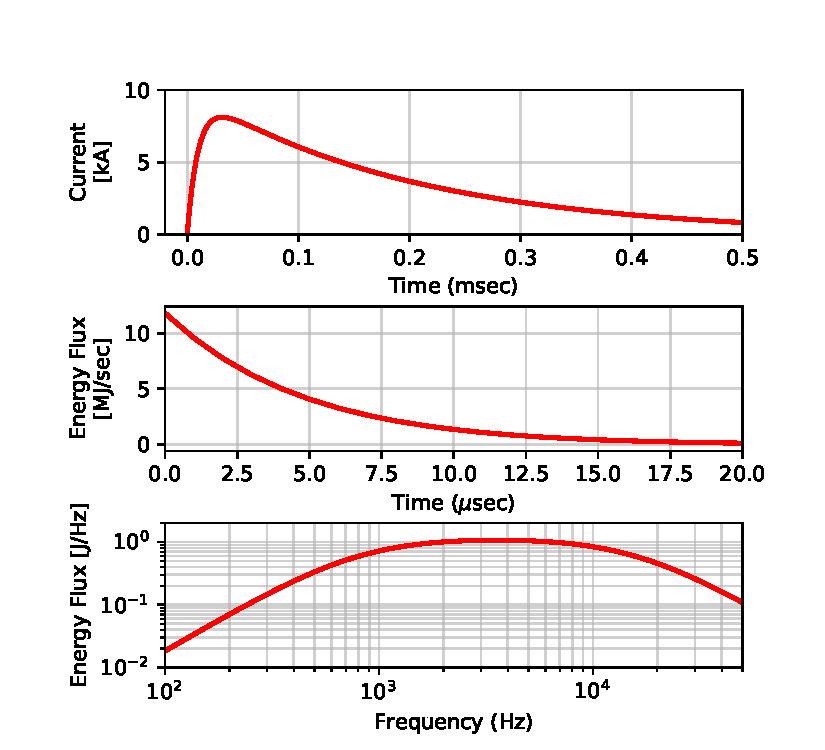
\includegraphics{figures/Lightning_spectra.pdf}

\caption[Time and frequency profiles of the lightning illumination model]{Double-exponential current pulse model of a lightning stroke. The top panel shows the stroke current vs time; the middle panel shows the total energy flux, integrated over space, vs time; the bottom panel shows the energy flux in the frequency domain.}
\label{fig:lightning_spectrum}
\end{center}
\end{figure*}
